% Options for packages loaded elsewhere
\PassOptionsToPackage{unicode}{hyperref}
\PassOptionsToPackage{hyphens}{url}
%
\documentclass[
]{book}
\title{The Ethical Dilemma of Producing Artificial Intelligence (AI)}
\author{Zach Gooding, Nisarg Jhaveri, Catherine Visscher, William Yu, Aaron Zhao}
\date{08-16-2023}

\usepackage{amsmath,amssymb}
\usepackage{lmodern}
\usepackage{iftex}
\ifPDFTeX
  \usepackage[T1]{fontenc}
  \usepackage[utf8]{inputenc}
  \usepackage{textcomp} % provide euro and other symbols
\else % if luatex or xetex
  \usepackage{unicode-math}
  \defaultfontfeatures{Scale=MatchLowercase}
  \defaultfontfeatures[\rmfamily]{Ligatures=TeX,Scale=1}
\fi
% Use upquote if available, for straight quotes in verbatim environments
\IfFileExists{upquote.sty}{\usepackage{upquote}}{}
\IfFileExists{microtype.sty}{% use microtype if available
  \usepackage[]{microtype}
  \UseMicrotypeSet[protrusion]{basicmath} % disable protrusion for tt fonts
}{}
\makeatletter
\@ifundefined{KOMAClassName}{% if non-KOMA class
  \IfFileExists{parskip.sty}{%
    \usepackage{parskip}
  }{% else
    \setlength{\parindent}{0pt}
    \setlength{\parskip}{6pt plus 2pt minus 1pt}}
}{% if KOMA class
  \KOMAoptions{parskip=half}}
\makeatother
\usepackage{xcolor}
\IfFileExists{xurl.sty}{\usepackage{xurl}}{} % add URL line breaks if available
\IfFileExists{bookmark.sty}{\usepackage{bookmark}}{\usepackage{hyperref}}
\hypersetup{
  pdftitle={The Ethical Dilemma of Producing Artificial Intelligence (AI)},
  pdfauthor={Zach Gooding, Nisarg Jhaveri, Catherine Visscher, William Yu, Aaron Zhao},
  hidelinks,
  pdfcreator={LaTeX via pandoc}}
\urlstyle{same} % disable monospaced font for URLs
\usepackage{longtable,booktabs,array}
\usepackage{calc} % for calculating minipage widths
% Correct order of tables after \paragraph or \subparagraph
\usepackage{etoolbox}
\makeatletter
\patchcmd\longtable{\par}{\if@noskipsec\mbox{}\fi\par}{}{}
\makeatother
% Allow footnotes in longtable head/foot
\IfFileExists{footnotehyper.sty}{\usepackage{footnotehyper}}{\usepackage{footnote}}
\makesavenoteenv{longtable}
\usepackage{graphicx}
\makeatletter
\def\maxwidth{\ifdim\Gin@nat@width>\linewidth\linewidth\else\Gin@nat@width\fi}
\def\maxheight{\ifdim\Gin@nat@height>\textheight\textheight\else\Gin@nat@height\fi}
\makeatother
% Scale images if necessary, so that they will not overflow the page
% margins by default, and it is still possible to overwrite the defaults
% using explicit options in \includegraphics[width, height, ...]{}
\setkeys{Gin}{width=\maxwidth,height=\maxheight,keepaspectratio}
% Set default figure placement to htbp
\makeatletter
\def\fps@figure{htbp}
\makeatother
\setlength{\emergencystretch}{3em} % prevent overfull lines
\providecommand{\tightlist}{%
  \setlength{\itemsep}{0pt}\setlength{\parskip}{0pt}}
\setcounter{secnumdepth}{5}
\usepackage{booktabs}
\ifLuaTeX
  \usepackage{selnolig}  % disable illegal ligatures
\fi
\usepackage[]{natbib}
\bibliographystyle{plainnat}

\begin{document}
\maketitle

{
\setcounter{tocdepth}{1}
\tableofcontents
}
\hypertarget{introduction}{%
\chapter{Introduction}\label{introduction}}

This website is a learning tool for the Ross community, including students, alumni, faculty, and staff, on the ethical issues of how we produce and generate artificial intelligence. The information book will first begin with team introductions then discuss a general introduction into the current production/generation of artificial intelligence.

After these introductions, we will transition into the main section of the book, discussing several areas of ethical concern as it relates to As artificial intelligence (AI) continues its integration into various facets of society, it becomes imperative to critically assess the ethical implications surrounding its development and usage. This website serves as a learning tool for the Ross community to explore key ethical considerations in the AI landscape, with a focus on large language models.

Before jumping into content, we will introduce the team that put this resource together for your education purposes.

At its core, this resource aims to unpack pressing ethical issues in AI advancement. We will begin by analyzing the substantial infrastructure and resources needed to create increasingly complex AI models and assessing environmental and financial costs. Moving forward, we will discuss crucial data-related factors, including unauthorized scraping and ingrained biases.
Additionally, this website will address inherent challenges in training ethical, safe AI systems. It will also stress the importance of responsible data handling and privacy measures taken by AI companies. Risks of misalignment between AI and human values will similarly be explored.

To conclude, we will overview two domains - personalized AI and open-source projects - that underscore AI's societal benefits despite its problems. Overall, we hope to spur thoughtful discussion about establishing ethical frameworks to guide AI progress in a way that prioritizes privacy, ensures security, and promotes human-centric values. This introduction sets the stage for an examination of AI ethics tailored to the Ross community.

\hypertarget{about-us}{%
\chapter{About Us}\label{about-us}}

Hi there, we are the Insight Titans! We are part of the Masters of Business Analytics Cohort Class of 2024. We are excited to share some helpful information with you that we hope you find useful for learning, just as we did in creating this resource.

\hypertarget{zach-gooding}{%
\section{Zach Gooding}\label{zach-gooding}}

Hello everyone! My name is Zach Gooding, and I am originally from Westmont, Illinois, a Western Suburb of Chicago. I graduated from Augustana College in the Spring of 2023 with majors in Data Analytics and Business Administration with concentrations in Marketing, Management, and MIS. I was also a four year member of the Varsity Baseball team at Augustana and was a part of back to back Conference Championship teams. My undergraduate experience made me realize I was just beginning to scratch the surface in the field of Data Analytics, so I am thrilled to be taking classes at Michigan Ross to further my education.

My prior work experience is as a Marketing and Data Analytics Intern for the NTT INDYCAR Series and Canes Baseball in their Illinois Division. In my free time, you can find me watching the Cubs game, listening to a lot of music, and experiencing everything Ann Arbor has to offer. I hope you find our information useful on Large Language Models as we enter this new age of Data.

\hypertarget{nisarg-jhaveri}{%
\section{Nisarg Jhaveri}\label{nisarg-jhaveri}}

Hey-o! I am Nisarg Jhaveri, an enthusiast from Boston, MA, and an auditor by profession. I completed my undergrad at the University of Massachusetts Lowell in Finance and Accounting with a minor in Psychology. I did five internships during that time frame to explore different industries. I graduated back in 2022, after which I worked at EY for a year with their Wealth and Asset Management team, but I kept itching to go back to school to learn more about programming, a topic that I couldn't fully explore.
I decided to join the Ross School of Business because of this and hope to make the most out of it to truly leverage data and create value while working on a few personal projects.
P.S. I am a very social person so feel free to reach out, I would love to chat/help :)

\hypertarget{catherine-visscher}{%
\section{Catherine Visscher}\label{catherine-visscher}}

Hello! I am Catherine Visscher, a Michigan native from Livonia, Michigan. I graduated from the University of Michigan College of Engineering Winter 2023 with a B.S.E in Chemical Engineering and am currently a Master's of Business Analytics student at the Stephen M. Ross School of Business. One thing my undergraduate degree has taught is how to break large, complex processes into more manageable components. I have experience as an engineer intern within the utility sector working at Consumers Energy, with work focused in root cause analysis and process optimization.

I am entering my fifth year as a member of the Women's Track and Field team at Michigan as a pole vaulter. Within the last year, we have been fortunate enough to win back-to-back Big Ten Conference Titles and I cannot wait for another season with this amazing team! In my somewhat limited free time, I enjoy reading and spending time with friends and family.

I hope the information we've gathered on artificial intelligence and how it is being generated is helpful to the current and future Ross community!

\hypertarget{william-yu}{%
\section{William Yu}\label{william-yu}}

Hello everyone, my name is William Yu and I am from China. I graduated from Indiana University Bloomington in 2022 majoring in Information Systems and Business Analytics. During my undergraduate studies, I had four internships with some consulting and technology firms such as IQVIA and TikTok. I also worked as a research assistant with a professor at the Kelley School of Business, Indiana University, focusing on the impact of dismantling coal power plants on the surrounding environment, economy and housing prices. These experiences game me valuable skills with data analysis helped me pratice my knowledge with some programming and data analysis tools, such as Python, SQL and R. After graduation, I want to find a quantitative analyst position in some financial firms because I want to be at the forefront of leveraging cutting edge quantitative techniques and mathematical models to solve complex financial problems,

During my free time, I am enthusiastic about cycling and triathlon. As a two time Ironman 70.3 finisher, I enjoy pushing myself beyond what I thought possible and the sense of accomplishment after every long-distance endurance workouts.

\hypertarget{aaron-zhao}{%
\section{Aaron Zhao}\label{aaron-zhao}}

Hey there, I'm Aaron! I studied in San Diego, California for my undergraduate degree, and since then, I've taken four epic trips from the West Coast to the East Coast, exploring new places and cultures along the way.

When I'm not studying for my degree, I love working with wood and 3D printing to make cool and useful stuff that brings joy to myself and others. My creative pursuits extend to the kitchen, where I enjoy experimenting to come up with delicious and creative meals. In my free time, I cherish simple pleasures like indulging in cookies and creme ice cream or savoring the delightful sashimi plate.

Psychology has always fascinated me because understanding why people do what they do feels like solving an exciting puzzle.

Alongside my academic and creative passions, I have three adorable and playful chinchillas, which inspire me to craft special things for them to enjoy.

Moreover, sharing knowledge is something I'm truly passionate about. During my undergraduate years, I loved being a teaching assistant, helping others learn and grow. It's an incredibly rewarding experience to see others flourish through my help.

\hypertarget{hardware}{%
\chapter{Hardware}\label{hardware}}

Hardware plays a crucial role in the development of AI Large Language Models (LLMs), as it influences the speed and effectiveness of the model's learning process. Additionally, the nature, size, intricacy, and objective of the model dictate its hardware needs. Key hardware components for AI training include: Processor (CPU) \& Graphic Card (GPU), Memory (RAM) \& Storage (Hard Drives) and Interconnects.

\hypertarget{case-analysis---chatgpt}{%
\section{Case Analysis - ChatGPT}\label{case-analysis---chatgpt}}

ChatGPT has purchased over 10,000 high-quality NVIDIA GPUs, boosting Nvidia product sales to between \$3 billion and \$11 billion annually. Among the GPUs, the NVIDIA A100 HPC \footnote{\url{https://privacytools.seas.harvard.edu/differential-privacy}} stands out, priced at \$12,500. It's a top-notch GPU with 80GB of HBM2 memory, providing up to 2TBps memory bandwidth, ideal for running massive models and datasets. However, even with this GPU, there are hurdles in enhancing AI training. For instance, when using PyTorch on a server with multiple GPUs, ChatGPT can only run smaller models like GPT-L due to its complexity and memory fragmentation. As a result, expanding its operation to 4 or 8 GPUs doesn't significantly improve performance. For memory and storage, ChatGPT relies on a mix of technologies such as HBM, SSDs, and Cloud State. Furthermore, it uses PCI Express, NVLink, and Ethernet for connectivity. The estimated daily cost for OpenAI to run these systems is around \$700,000 \footnote{\url{https://www.intelligence.gov/principles-of-artificial-intelligence-ethics-for-the-intelligence-community}}.

\hypertarget{case-analysis---bard}{%
\section{Case Analysis - Bard}\label{case-analysis---bard}}

In contrast to Bard, another of Google's AI products which uses the GPU provided by NVIDIA, Google employed its own hardware to develop the PaLM model. As of April 2023, Google announced that they had constructed a system consisting of over 4,000 TPUs, complemented by bespoke components engineered specifically for running and training AI models. This system has been operational since 2020 and was the powerhouse behind the training of Google's PaLM model, a rival to OpenAI's GPT, over a span of 50 days. Google researchers have highlighted that their TPU-based supercomputer, dubbed TPUv4, boasts a performance that is between 1.2 to 1.7 times faster and consumes between 1.3 to 1.9 times less energy compared to the Nvidia A100\footnote{\url{https://venturebeat.com/ai/redpajama-replicates-llama-to-build-open-source-state-of-the-art-llms/}}, and this model has cost Google \$100 billion to develop\footnote{\url{https://huggingface.co/docs/transformers/philosophy}}.

\hypertarget{ethical-dilemmas}{%
\section{Ethical Dilemmas}\label{ethical-dilemmas}}

\hypertarget{resource-allocation}{%
\subsection{Resource Allocation}\label{resource-allocation}}

The immense computational power needed to train large AI models requires significant financial investment. As we can see in the chart below\footnote{\url{https://research.netflix.com/research-area/machine-learning}} \footnote{\url{https://www.nature.com/articles/s41591-023-02448-8}}, the training cost for AI model development has been constantly increasing, and it is predicted to grow exponentially in the following years. The concern arises when considering how these resources might be alternatively used to address pressing societal issues like healthcare, education, infrastructure, or poverty reduction. Also, the allure of cutting-edge AI research may divert talent and funding away from other vital scientific areas. This can create an imbalance in research fields, possibly neglecting areas that might have a more immediate positive impact on human well-being.

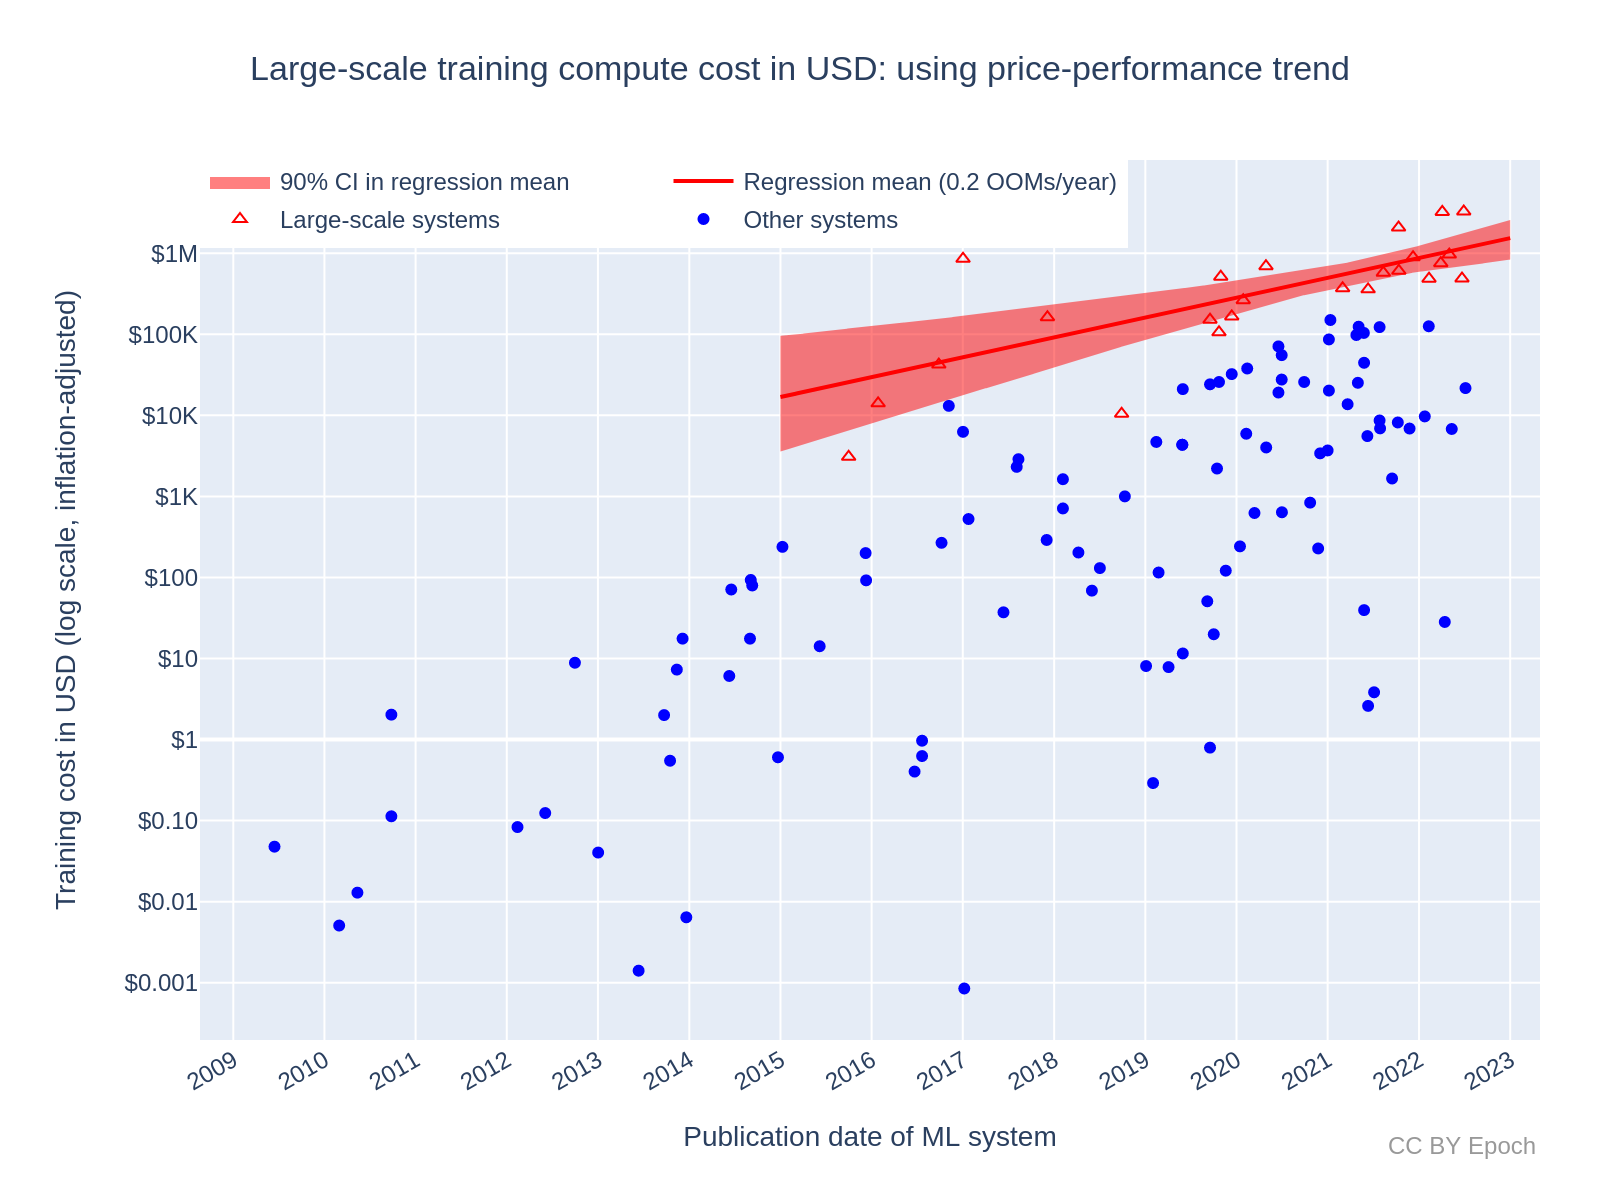
\includegraphics{figures/figure1.png}
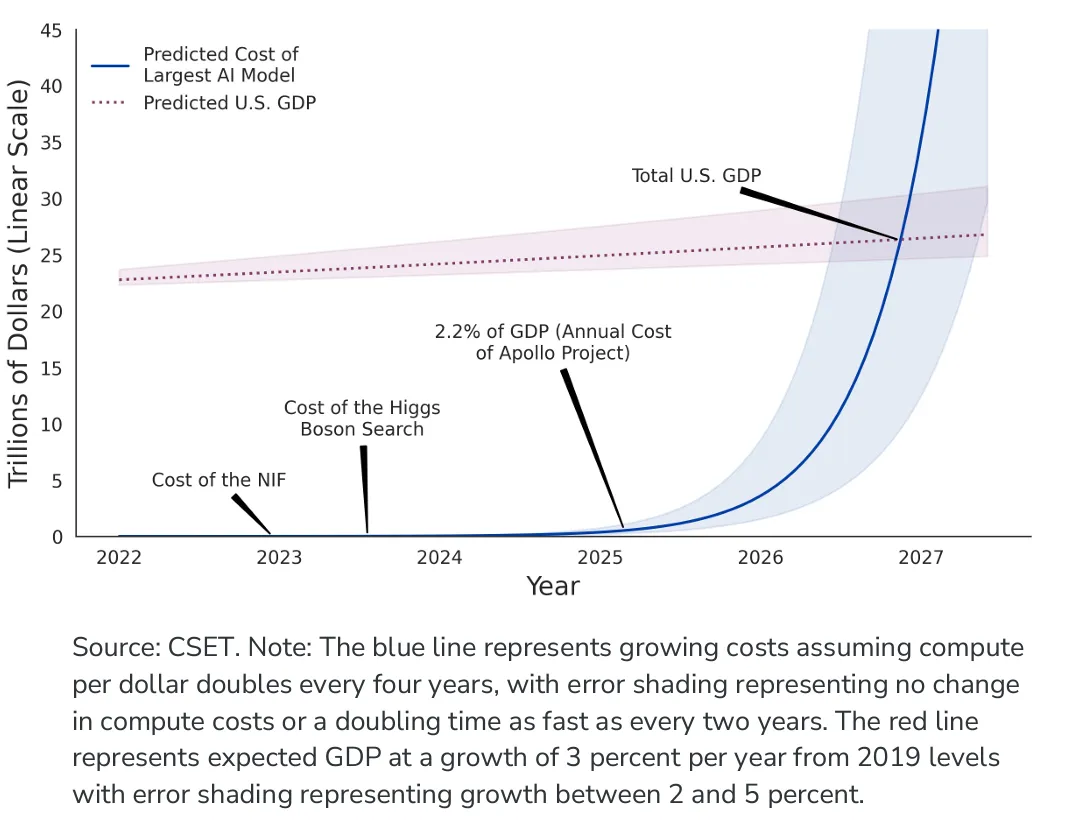
\includegraphics{figures/figure2.png}
\#\#\# E-Waste
The surge in the development of AI Large Language Models (LLMs) has resource implications that can be likened to the cryptocurrency boom two years ago, with its consequent mass production of electronic waste. The following chart\footnote{\url{https://www.cancer.gov/news-events/cancer-currents-blog/2022/artificial-intelligence-cancer-imaging}} shows the significant increase in Bitcoin Electronic Waste Generation over the past five years. The development of large AI language models, like cryptocurrency mining, requires substantial equipment investment and relatively frequent equipment iteration and upgrades. After each round of equipment upgrades, the original devices become obsolete and ultimately end up as electronic waste. Moreover, considering the specific functionality of the hardware used in large AI language models, there is even less hardware that can be recycled compared to the hardware discarded from mining.

\begin{figure}
\centering
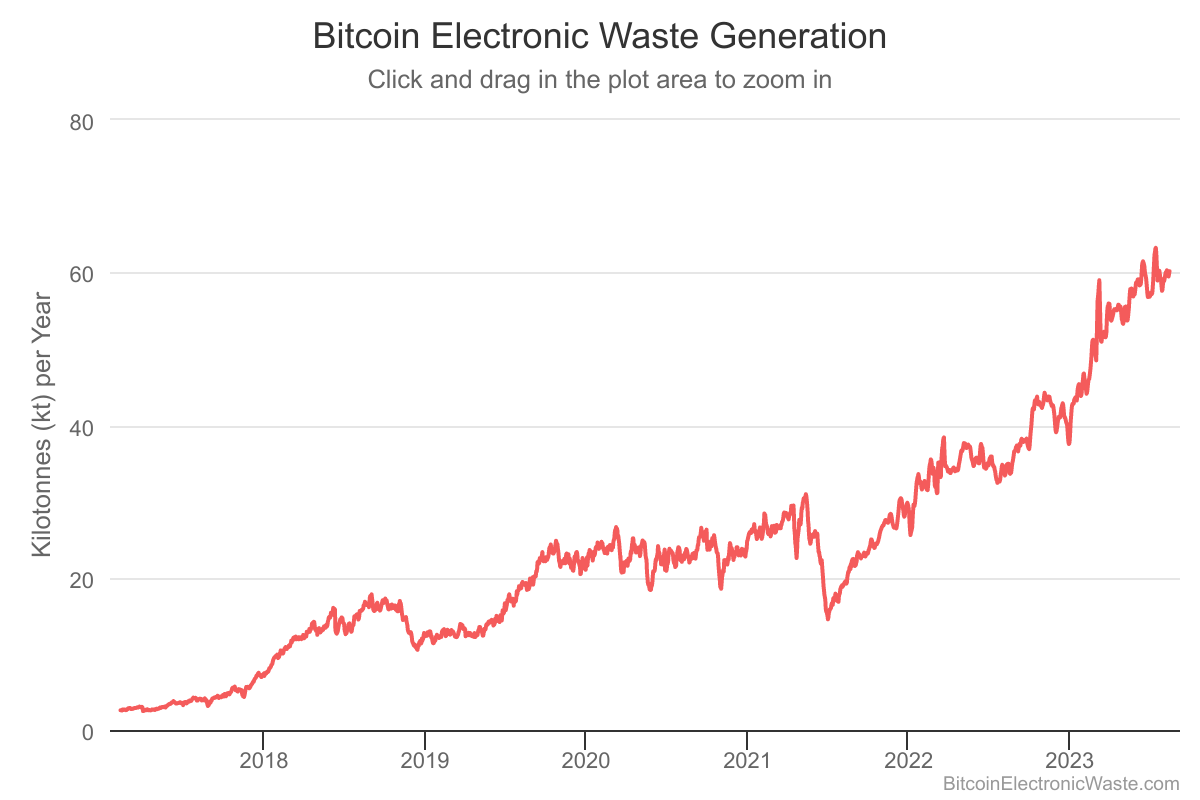
\includegraphics{figures/figure3.png}
\caption{Estimated Cost of Compute}
\end{figure}

\hypertarget{natural-resource-consumption}{%
\chapter{Natural Resource Consumption}\label{natural-resource-consumption}}

One part of producing large artificial intelligence models that many users do not think of is the energy and water it takes to train these models and run them before they are available to the masses. As AI models get increasingly larger, companies will have to be more conscious of the energy required to make them, especially as the world moves towards a more carbon-neutral future.

\hypertarget{facts-on-current-generative-ai-energy-usage}{%
\section{Facts on Current Generative AI Energy Usage}\label{facts-on-current-generative-ai-energy-usage}}

Gauging how much energy generative AI uses can be difficult for everyday users unfamiliar with the scale of energy units such as kilowatt hours or watts. There are several comparisons between the amount of energy it takes to train these models to things people are more familiar with. This includes comparisons such as power going to homes, as well as carbon dioxide emissions of an average American car. Some facts are listed below.

\begin{itemize}
\item
  Just one model's training can use more electricity than 100 US homes in a year\footnote{\url{https://news.umich.edu/new-language-learning-algorithms-risk-reinforcing-inequalities-social-fragmentation-per-u-m-study/}}.
\item
  Training just one AI model can emit more than 626,000 pounds of carbon dioxide equivalent, which is nearly 5 times the lifetime emissions of an average American car\footnote{\url{https://news.emory.edu/stories/2022/05/hs_ai_systems_detect_patient_race_27-05-2022/story.html}, \url{https://www.thelancet.com/journals/landig/article/PIIS2589-7500(22)00063-2/fulltext}}.
\item
  ``Training the GPT-3 model just once consumes 1,287 MWh, which is enough to supply an average U.S. household for 120 years.''\footnote{\url{https://blog.twitter.com/engineering/en_us/topics/insights/2021/learnings-from-the-first-algorithmic-bias-bounty-challenge}}
\item
  Generating a single AI model with 110 million parameters consumed the energy required for a round-trip transcontinental flight for one person\footnote{\url{https://www.scientificamerican.com/article/a-computer-scientist-breaks-down-generative-ais-hefty-carbon-footprint/}}.
\end{itemize}

Some may argue that training any computer models takes large amounts of energy, but because AI programs are so complex, they require more energy than other forms of computing\footnote{\url{https://www.theguardian.com/technology/2023/jun/08/artificial-intelligence-industry-boom-environment-toll}}. Seeing the comparisons made to everyday objects emphasizes the environmental impact of these models and how things need to change.

\hypertarget{why-training-generative-ai-uses-so-much-energy}{%
\section{Why Training Generative AI Uses So Much Energy}\label{why-training-generative-ai-uses-so-much-energy}}

There are many predictors of carbon emissions for these large AI models. Size is one of them, which includes the number of parameters a model has. Creating GPT-3, which has 175 billion parameters, generated an estimated 552 tons of carbon dioxide equivalent as it consumed 1,287 megawatt hours of electricity. As AI evolves, the number of parameters increases, with GPT-4 having over 1.7 trillion parameters. Below is a table of energy consumption of some large deep learning models\footnote{\url{https://medium.com/mlearning-ai/rethinking-large-language-models-for-nlp-alternatives-and-efficiency-73c6fead5ebf}}

\begin{figure}
\centering
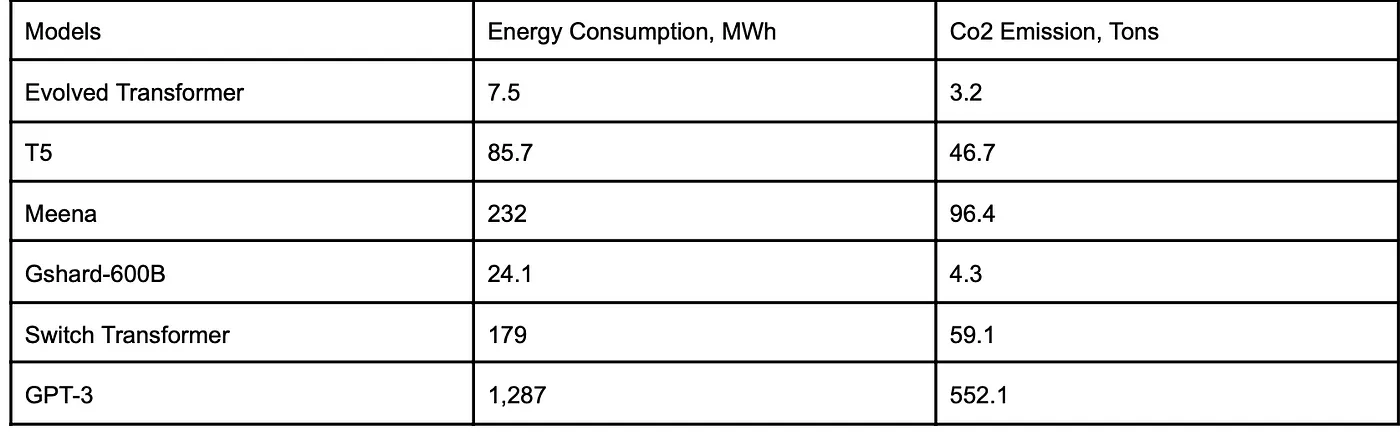
\includegraphics{figures/figure4.png}
\caption{Energy Consumption of Some Large Deep Learning Models}
\end{figure}

This emphasizes the fact that size has a huge impact on the energy consumption of these models. Meena, which is a model being created by Google ventures, has 2.6 billion parameters, and training it consumes only 18\% of the energy that training GPT-3 does. As models continue to grow, developers will need to keep this in mind as we move away from fossil fuels as a primary energy resource.

\hypertarget{ais-water-consumption}{%
\section{AI's Water Consumption}\label{ais-water-consumption}}

One other main area of natural resource concern in training and running AI is the water consumption of these large models. We have already discussed the large amounts of energy these models require, but with these high-energy systems come high operating temperatures. This is where freshwater comes in, an increasingly scarce natural resource needed to cool these complex systems and keep the entire infrastructure running at an acceptable temperature\footnote{\url{https://www.businessinsider.com/chatgpt-generative-ai-water-use-environmental-impact-study-2023-4}}. Researchers at the University of California, Riverside found that training for a GPT-3 model at Microsoft's cutting edge data center consumed 700,000 liters of freshwater. This is equivalent to the same amount of water used to manufacture around 320 Tesla electric vehicles\footnote{\url{https://news.ucr.edu/articles/2023/04/28/ai-programs-consume-large-volumes-scarce-water}}. The same group found that using 20-50 AI queries can use roughly half a liter of freshwater, an already scarce resource. Saltwater cannot be used to replace these water-wasting systems because it can lead to corrosion, clogged water pipes, and bacterial growth. Many believe that as AI continues to evolve and grow bigger, so will its water consumption. It is hard to fully gauge the actual water footprint of these large models but companies will have to reevaluate their sustainability goals as AI is becoming more and more integrated into our daily lives.

\hypertarget{how-companies-can-make-ai-models-greener}{%
\section{How Companies Can Make AI Models Greener}\label{how-companies-can-make-ai-models-greener}}

A study done by Google found that for the same size model, using a more efficient model architecture and processor with greener data centers can reduce the carbon footprint of these models by 100 to 1,000 times\footnote{\url{https://ai.googleblog.com/2022/02/good-news-about-carbon-footprint-of.html}}. This study was specific to machine learning, but this movement towards more efficient smaller models could be the way companies produce AI with a smaller environmental footprint. Google has found the 4Ms which are the best practices to reduce energy and carbon footprints. The four Ms are model, machine, mechanization, and map optimization. They are broken down further below.

\begin{itemize}
\tightlist
\item
  Model: Selecting more efficient models, such as sparse models which can advance model quality and reduce computation.
\item
  Machine: Using processors/systems of optimized training for models which can improve performance and energy efficiency.
\item
  Mechanization: Computing in the cloud with warehouses equipped for energy efficiency.
\item
  Map optimization: Allows users to pick locations with the cleanest energy.
\end{itemize}

Google believes that the 4Ms used together can reduce energy and emissions by 100x. With the 4Ms in mind, software developers working on future AI models can hopefully find areas to optimize and slim down their models to match the carbon-neutrality path we are moving towards to support a sustainable future.

\hypertarget{data}{%
\chapter{Data}\label{data}}

Data collection is the foundational step in the development of AI Large Language Models. The model's accuracy and effectiveness heavily rely on the quality and origin of this data. Data comes from two primary sources: open-source datasets and independent content websites\footnote{\url{https://privacytools.seas.harvard.edu/differential-privacy}}. The former, open-source data, such as Wikipedia, consists of large amounts of data usually accessible for commercial use, including the training of LLMs. On the other hand, independent content websites -- such as news publications like The Washington Post or The Wall Street Journal, creator-focused platforms like Patreon or Medium, and user-driven platforms like Reddit or Twitter -- tend to have stricter policies. These sites are more protective about their content, particularly against unauthorized scraping for commercial applications.

The table below shows the composition of a dataset called C-4, which Google used for its AI model training. However, with the popularity of the AI LLM, there are growing concerns about data, especially in terms of data content and collection methods.

\begin{figure}
\centering
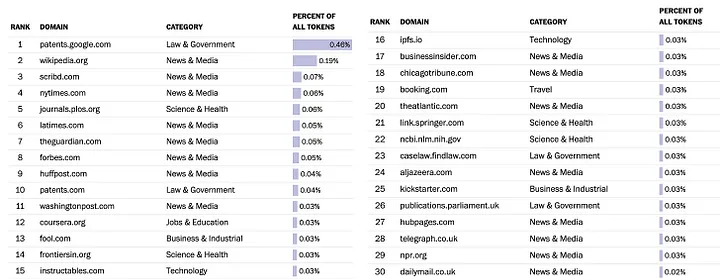
\includegraphics{figures/figure5.png}
\caption{Top 30 Sources for C-4 Dataset}
\end{figure}

\hypertarget{diversitybiases-of-data}{%
\section{Diversity/Biases of Data}\label{diversitybiases-of-data}}

A major concern about the quality of data used in training AI Large Language Models is ensuring that this data is diverse and free of bias. Given that a significant portion of the training data for these models comes from public sources, guaranteeing impartiality is challenging. For instance, Amazon encountered bias with an NLP tool designed to screen job applicants' resumes. The tool was trained on past resumes, using their linguistic patterns to filter current candidates. Historically, resumes from women were underrepresented, the tool unintentionally favored male candidates \footnote{\url{https://www.intelligence.gov/principles-of-artificial-intelligence-ethics-for-the-intelligence-community}}.

Similarly, a study analyzing 800 billion words from the internet highlighted that certain demographics, especially African Americans, were frequently associated with negative terms. Notably, there were evident biases against senior citizens and individuals with disabilities. Systems like ChatGPT, which derive their knowledge from the vast expanse of the internet, risk mirroring these biases. Such risks are further exacerbated if someone deliberately tries to manipulate the model to disseminate false or biased information. As AI models become more integral to various sectors, addressing these biases is crucial to ensure fair and unbiased decision-making.

\hypertarget{web-scraping}{%
\section{Web Scraping}\label{web-scraping}}

One of the major concerns with data collection is web scraping. Ideally, LLM developers should maintain transparency by clearly identifying their data sources and ensuring that their scraping practices adhere to the content owners' terms of use. Unfortunately, this has not always been the case, leading to concerns about data privacy and intellectual property rights. OpenAI has been facing criticism for its alleged lack of transparency concerning its data collection methods. The C-4 dataset mentioned above seems to have mostly relied on web scraping, and in some instances, these scraping activities may have contravened the content owners' terms.

An illustrative example of these challenges is Reddit's policy change in April 2023 regarding its API, which had been freely accessible since 2008 \footnote{\url{https://venturebeat.com/ai/redpajama-replicates-llama-to-build-open-source-state-of-the-art-llms/}}. The decision was prompted by the actions of Pushshift, a data aggregation site commonly utilized by LLM developers. Pushshift's practices had reportedly violated Reddit's API rules, leading to the policy revision. Such incidents underscore the need for clear guidelines when collecting training data from independent content websites.

\hypertarget{intellectual-property}{%
\section{Intellectual Property}\label{intellectual-property}}

Intellectual Property protection is another concern with data collection. With tools like ChatGPT that can learn from user inputs, there is a potential threat to proprietary information. If users inadvertently or carelessly input sensitive details, it could jeopardize their company's confidential data or intellectual property. A noteworthy instance is the case of Samsung employees who mistakenly shared proprietary data while using ChatGPT as a work aid, culminating in a substantial data breach\footnote{\url{https://huggingface.co/docs/transformers/philosophy}}.

In 2022, Microsoft, GitHub, and OpenAI faced a proposed class-action lawsuit over ``software piracy'' in relation to their AI tool, GitHub Copilot. Trained on vast swathes of public code repositories, the tool has come under scrutiny for allegedly replicating extensive segments of copyrighted code without appropriate credit\footnote{\url{https://research.netflix.com/research-area/machine-learning}}.

\hypertarget{bias}{%
\chapter{Bias}\label{bias}}

Humans are referred to by many in the data field as the most advanced form of Artificial Intelligence (AI) and Large Language Models (LLM). Yes, as these two big data concepts have become more commonplace in society today; data analysts, scientists, professionals, and students alike have all relied on the use of AI and LLMs at some point for a specific purpose. However, what makes people more advanced than AI and LLMs is intuition and context. These are two soft, intangible things LLMs cannot possess.

\hypertarget{the-subtle-bias-in-training-data}{%
\section{The Subtle Bias in Training Data}\label{the-subtle-bias-in-training-data}}

Anees Merchant, Head of Global Growth and Client Success - Digital, Applied AI, and Research at Core5 Intelligence expands on this notion of bias in LLMs in a post on his personal blog titled ``Large Language Models and Bias: An Unresolved Issue''. Within this blog post, Merchant discusses the fact that bias ``can be as subtle as a model associating certain occupations with a specific gender or as blatant as a model generating offensive or harmful content.'' In simple terms, LLMs when prompted will associate Doctor to being a male occupation and Nurse to being a female occupation. How does this happen? It has everything to do with the data that these models are trained on. According to Merchant, ``if the training data contains biased information, the model will inevitably learn and reproduce these biases.'' The problem with this is that it can perpetuate harmful stereotypes and discrimination. For example, if an LLM is used as a hiring tool in an engineering field, it may put female applicants at a disadvantage \footnote{\url{https://privacytools.seas.harvard.edu/differential-privacy}}.

\hypertarget{mit-study}{%
\section{MIT Study}\label{mit-study}}

In a study performed by MIT on the popular Large Language Model ChatGPT, when prompted about bias, the response is, ``Yes, language models can have biases, because the training data reflects the biases present in society from which that data was collected. For example, gender and racial biases are prevalent in many real-world datasets, and if a language model is trained on that, it can perpetuate and amplify these biases in its predictions''. There within itself is the primary issue. Although ChatGPT has the awareness to understand its biased tendencies, due to the way it is programmed, it cannot produce answers that mitigate bias. According to the researchers at MIT, ``current language models suffer from issues with fairness, computational resources, and privacy''. The research conducted also returned the conclusion that ``language models have similar properties. A language model without explicit logic learning makes plenty of biased reasoning, but adding logic learning can significantly mitigate such behavior'' \footnote{\url{https://www.intelligence.gov/principles-of-artificial-intelligence-ethics-for-the-intelligence-community}}.

\hypertarget{addressing-the-issue}{%
\section{Addressing The Issue}\label{addressing-the-issue}}

The question now becomes how do we address the issue? Referencing the first source, while there is no clear answer, Merchant suggests that it is a combination of technical and non-technical approaches and the involvement of various stakeholders. They will then attempt to develop methods during the model training process that aims to reduce the influence of biased patterns in training data. It is important from a non-technical perspective to have diverse teams working on the development and deployment of LLMs. There is, however, an education piece addressing the issue as well. According to Merchant, transparency and interpretability are crucial. Understanding and explaining how a model makes decisions can help identify and mitigate bias.

\hypertarget{hallucinations}{%
\section{Hallucinations}\label{hallucinations}}

Another layer to the biases within Large Language Models is hallucinations. A hallucination refers to the phenomenon where the model generates text that is incorrect, nonsensical, or not real. This is because LLMs are not databases or search engines; therefore they cannot cite what their response is based on. A very basic example of hallucinations in LLMs is building a two-letter bigrams Markov model from text. As the model begins to pull out the two-letter bigrams from the text, the probabilities change because of the statistical patterns. Eventually, when prompted by a letter, the LLM will return a word it invented that does not exist. Hallucinations are caused by ``limited contextual understanding since the model is obligated to transform the prompt and the training data into an abstraction'' \footnote{\url{https://venturebeat.com/ai/redpajama-replicates-llama-to-build-open-source-state-of-the-art-llms/}}.

\hypertarget{alignment}{%
\chapter{Alignment}\label{alignment}}

By its very definition, we are seeking to have AI understand and remain in line with human interests as the systems become more capable and autonomous. Working with limited sets of data, the alignment becomes particularly important as we need to prevent unintended negative consequences or risks. Human values, as previously mentioned, are ever-evolving and can have various interpretations for any given scenario based on the context of a particular culture. This brings us to our list of issues with alignment: what is the desired specification of human value? Can AI learn and generalize values based on a training dataset that may be different? Can we have AI stick to the values for the longer-term/not drift away from human-centric values? And lastly, can algorithms improve over time?

\hypertarget{value-alignment}{%
\section{Value Alignment?}\label{value-alignment}}

What values are AI supposed to align with? We can consider two schools of thought here, one where we take a single user and ensure that the model is aligned with their perspective, i.e., self-driving or autonomous vehicles where there is only one driver and we want to make sure that the vehicle is only listening to commands from the user and doesn't do its own thing. The other perspective is more along the lines of a global alignment with the entire human race so we do not have a catastrophic event occur or create risks on that level. However, most cases tend to fall under the gray area between the two where we have multiple people with diverse groups of users and thus subsets of humanity in general. This essentially ends up creating overlapping values but conflicting interests. With diverse groups, we have yet another loop of issues, are all values considered equal, or do you train your LLM to value one over the other?

With the emergence of these questions, one would normally expect the AI system to mimic and align itself in a manner of current human societies and follow a complex hierarchy based on status, power, wealth, and influence which would seem improbable, not to mention highly unethical - essentially bringing us back to square one. A suggestive approach might be to implement a general cooperative inverse reinforcement learning model where certain responses are punished and removed from the model. However, the conflict of interests would soon make the CIRL model inefficient or ineffective as it slowly complicates itself. \footnote{\url{https://privacytools.seas.harvard.edu/differential-privacy}}

\hypertarget{generalizing-values}{%
\section{Generalizing Values}\label{generalizing-values}}

Imagine a scatter plot, one of the most basic ones with a linear progression displaying a certain slope on the chart. Then add a trendline to get the m from our basic y = mx + b equation. That trendline that was created is the equivalent of generalization in machine learning, as no matter where you try to place the line, you will still have points that are away from the trendline you have created.\footnote{\url{https://www.intelligence.gov/principles-of-artificial-intelligence-ethics-for-the-intelligence-community}}

Let's say you create a very complex model that takes into account all the data points on the chart. Now, we have a complicated system that is not only slower but also has one fatal flaw which would be its vulnerability to new data sets.\footnote{\url{https://venturebeat.com/ai/redpajama-replicates-llama-to-build-open-source-state-of-the-art-llms/}}

Ideally speaking, you want the model to be as simple as possible and then have the system predict a new sample of data, compare the new sample, and improve based on the differences. The basic assumptions are that the examples are independent and identical, the distribution is stationary - meaning the data doesn't change over time, and whenever the data is pulled, it is the same distribution for training, validation, and test sets.

As we would have already assumed, the assumptions are straightforward to break, especially with the stationary assumption, as user input is very inconsistent and can change over time. For instance, an online shopper might change their preferences as the seasons change or new things come into fashion.
To conclude on the biggest nightmare of data scientists across the globe: overfitting, incomplete data, and inaccurate data labels make it nigh impossible for the models to adapt to new data. Overfitting means that the parameters of the model are too specific to the current dataset, and inaccurate data labels cause difficulties in supervised learning while training AI models.

\hypertarget{drifting}{%
\section{Drifting}\label{drifting}}

Let's say we train this amazingly complex system that is in line with our expectations of generalized human values and can adapt to new data despite having a limited training dataset; the next step would be to ensure that the model doesn't ``drift.'' So what does drift mean? Drift is a term used to describe how a machine learning model's performance tends to get worse over time as the models lose their accuracy due to changes in the environment. The changes can happen as the training dataset is simply outdated, the model is being applied to a new context, or the desired output keeps changing with a wide distribution of input.\footnote{\url{https://huggingface.co/docs/transformers/philosophy}}

As one can imagine, this can be a big problem as the real world keeps changing and we can experience various types of drifts as the model tries to adapt to the changing environment and depending on the model's ability to handle new data we can notice different types of drifts.

\hypertarget{concept-drift5}{%
\subsection[Concept Drift]{\texorpdfstring{Concept Drift\footnote{\url{https://research.netflix.com/research-area/machine-learning}}}{Concept Drift}}\label{concept-drift5}}

\begin{figure}
\centering
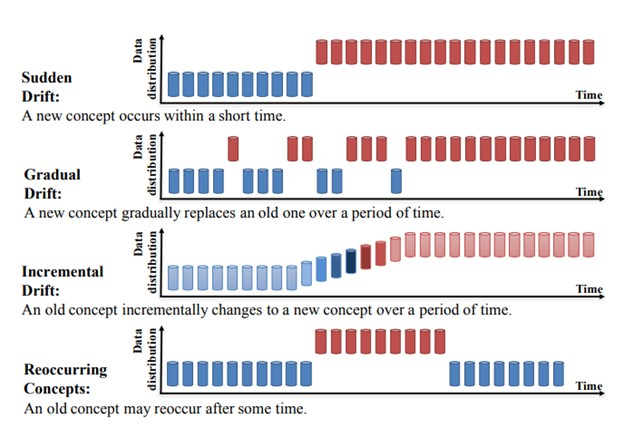
\includegraphics{figures/figure6.png}
\caption{Top 30 Sources for C-4 Dataset}
\end{figure}

The following explanations for various types of drift have been provided by ChatGPT:\footnote{\url{https://www.nature.com/articles/s41591-023-02448-8}}

\begin{itemize}
\item
  Sudden Drift: Sudden concept drift occurs when the underlying task experiences a rapid change. An example could be a sentiment analysis model that was trained on a corpus of online reviews. If a new trend or event significantly alters the language used in reviews, the model's effectiveness might diminish abruptly.
\item
  Gradual Drift: Gradual concept drift involves a slow shift in the underlying task. For instance, a weather forecasting model might face gradual drift as climate patterns evolve over time, requiring the model to adapt its predictions.
\item
  Incremental Drift: Incremental drift refers to gradual changes that accumulate over time, causing the
  model's performance to gradually decline. This type of drift is often encountered in scenarios where the task involves dynamic and evolving data.
\item
  Recurring Concepts: Recurring concept drift happens when patterns in the data repeat themselves periodically. In finance, for instance, economic cycles can cause models to experience recurring concept drift.
\end{itemize}

\hypertarget{data-drift}{%
\subsection{Data Drift}\label{data-drift}}

Data drift, also known as covariate shift, focuses on changes in the distribution of input data. This type of drift can impact a model's accuracy even when the task remains constant. An example would be a medical diagnosis model trained on data from a specific hospital. If the demographics of the patients change over time, the model might struggle to make accurate diagnoses.

With systems designed and in place for the detection of any form of drifting, we can quickly and efficiently reinforce our models to provide desired outputs for these commonly occurring drifts.

\hypertarget{algorithmic-improvement}{%
\section{Algorithmic improvement}\label{algorithmic-improvement}}

Self-improving AI is a concept that is not foreign to those who have been in the field for a while. Our current AI systems are limited and narrow; however, the long-term goal has always been aimed at creating a system of artificial general intelligence - AGI.\footnote{\url{https://www.cancer.gov/news-events/cancer-currents-blog/2022/artificial-intelligence-cancer-imaging}}

AGI systems can be a potential solution to this problem, as noted by Ramana Kumar, an AGI safety researcher at DeepMind, as this self-improvement capability would be an innate characteristic of AGI. So despite being a theoretically sound thing, what is stopping the creation of AGI? It is a matter of scaling.
We require the existing machine-learning models to be scaled up, for instance, with faster hardware. We can have incremental research progress for different forms of learning, such as representation, transfer, and model-based reinforcement. This form of recursive self-improvement allows the system to establish a feedback loop for making adjustments to its own functionality to improve performance. \footnote{\url{https://news.umich.edu/new-language-learning-algorithms-risk-reinforcing-inequalities-social-fragmentation-per-u-m-study/}}

\hypertarget{privacy}{%
\chapter{Privacy}\label{privacy}}

Privacy has been the poster child for problems with LLMs for quite some time now, especially when it comes to the privacy of one's personal information. There are two main obstacles that stand in the way of true privacy in LLMs: Infrastructure and IP protection. According to Daniel Huynh of Mithril Security, requirements for privacy in infrastructure are ``the hosting the model in specialized data centers, e.g., in the Cloud, removes the need for complex infrastructure. It becomes pretty easy to feed data to these models and get a result.'' As it relates to IP Protection, Huynh believes that ``it becomes much more challenging for AI consumers to steal the model's weights (notwithstanding model extraction attacks with a black-box API).'' \footnote{\url{https://privacytools.seas.harvard.edu/differential-privacy}}

\hypertarget{scaling-laws-specialized-data-centers-energy-impact}{%
\section{Scaling Laws \& Specialized Data Centers Energy Impact}\label{scaling-laws-specialized-data-centers-energy-impact}}

Mithril Security reflects on a trend discussed in a paper by a team of Computer Scientists at Cornell University called ``Scaling Laws for Neural Language Model,'' which was published in January of 2020. In this paper, the team is reporting their findings on the study of empirical scaling laws for language model performance on cross-entropy loss. The trend that is discussed is that it seems ``the loss scales as a power-law with model size, dataset size, and the amount of compute used for training.'' \footnote{\url{https://www.intelligence.gov/principles-of-artificial-intelligence-ethics-for-the-intelligence-community}} Daniel Huynh takes this scale of power-law and discusses how ``given the power requirements of those models, it also makes sense from an ecological perspective to rely on specialized data centers rather than on-premise deployment.'' Furthermore, ``economies of scale that Cloud providers leverage are more energy efficient than companies employing on premise.''

Referring back to the first source, this visualization shows how data centers have become increasingly energy efficient. Why Huynh emphasizes this energy efficiency in cloud hosting is because according to the team at Cornell, ``simple equations govern the dependence of overfitting on model/dataset size and the dependence of training speed on the model size''. Basically, cloud hosting is the simplest form of being able to handle the large-scale requirements of LLMs currently.

\hypertarget{cloud-hosting-privacy-enhancing-technologies}{%
\section{Cloud Hosting \& Privacy Enhancing Technologies}\label{cloud-hosting-privacy-enhancing-technologies}}

As it relates back to privacy in LLMs, cloud hosting comes with a cost. According to Mithril Security, ``sensitive data becomes potentially exposed to the actors providing those large models and the Cloud Provider.'' Unfortunately, given the current processes of these systems, sensitive data being potentially exposed can happen rather easily. ``If one actor (either the Cloud or the solution provider) is compromised or malicious, thousands of users' data can be exposed.'' Mithril Security is determined to lead the next steps in LLM production through Privacy Enhancing Technologies. Specifically, Mithril Security has a Privacy Enhancing Technology called BlindAI. BlindAI is ``an open-source solution to query and deploy AI models while guaranteeing data privacy. The querying of models is done via our easy-to-use Python library. How it works is ``data sent by users to the AI model is kept confidential at all times by hardware-enforced Trusted Execution Environments.'' There are two main uses for BlindAI: BlindAI API and BlindAI Core. BlindAI API is ``using BlindAI to query popular AI models hosted by Mithril Security.'' BlindAI Core is ``using BlindAI's underlying technology to host your own BlindAI server instance to securely deploy your own models.'' \footnote{\url{https://venturebeat.com/ai/redpajama-replicates-llama-to-build-open-source-state-of-the-art-llms/}} The visual below shows BlindAI in practice.

\hypertarget{automl}{%
\section{AutoML}\label{automl}}

Another current process for privacy in LLMs is AutoML. ``AutoML refers to the automated process of end-to-end development of machine learning models. It involves automating data preprocessing, feature selection, model selection, and hyperparameter tuning. It allows users with varying levels of expertise to develop machine-learning models with high efficiency and minimal manual intervention.'' There are several reasons to employ AutoML. First and foremost, ``organizations can maintain full control of their data.'' Obviously, keeping sensitive information in-house limits the transferring of information, thus reducing the chance it is exposed. According to Manuel Herranz, the CEO of Pangeanic, ``this approach ensures data privacy regulations compliance, a crucial aspect in sectors like healthcare, finance, and education, where stringent data privacy rules apply.'' Furthermore, self-training LLMs like AutoML ``reduces the dependency on external tech giants, providing more autonomy to organizations. \footnote{\url{https://huggingface.co/docs/transformers/philosophy}} BlindAI and AutoML are two different ways to increase privacy in the production of LLMs.

\hypertarget{personalized-large-language-models-llms}{%
\chapter{Personalized Large Language Models (LLMs)}\label{personalized-large-language-models-llms}}

\hypertarget{what-is-hugging-face}{%
\section{What is Hugging Face?}\label{what-is-hugging-face}}

Hugging Face holds a significant position within AI, open source, and machine learning domains. It plays a crucial role in shaping AI technology's landscape while promoting accessibility and democracy in AI. As a central hub, Hugging Face brings together tech-savvy individuals and general users, facilitating the collaborative construction of AI models like GPT-3 and BERT. These models undergo rigorous training on extensive datasets, enabling them to generate human-like textual content that has become a part of our daily lives.

However, Hugging Face's role goes beyond being a repository for these models and machine learning algorithms as it provides comprehensive toolkits for AI enthusiasts. The platform offers many resources and collaborative features that empower researchers and developers to integrate these models into their projects seamlessly. Whether for specific applications or scholarly investigations, as seen in recent work like the study conducted by UC Berkeley on GPT-4, Hugging Face equips people with the means to incorporate these advanced models effectively.

Therefore, understanding the significance of Hugging Face becomes crucial in the realm of personalized LLMs.

\hypertarget{democratizing-access}{%
\subsection{Democratizing Access}\label{democratizing-access}}

Hugging Face is prominent in democratizing AI technology, providing open access to meticulously researched and trained AI models. This accessibility empowers developers and researchers alike, sparing them the laborious task of constructing complex models from the ground up. Instead, they can focus their expertise where it matters most.

\hypertarget{accelerating-ai-development-pretrained-models-and-technological-partnerships}{%
\subsection{Accelerating AI Development: Pretrained Models and Technological Partnerships}\label{accelerating-ai-development-pretrained-models-and-technological-partnerships}}

Hugging Face further accelerates AI development through its diverse range of pre-trained models. These models facilitate rapid prototyping and streamline the implementation of AI solutions. By eliminating the need to build complex models from the ground up, Hugging Face allows developers and researchers to concentrate on refining their applications.\footnote{\url{https://privacytools.seas.harvard.edu/differential-privacy}}

Moreover, the platform has fostered meaningful partnerships with cutting-edge technologies such as Habana Gaudi---an innovative deep-learning training and inference processor. This collaboration is highlighted through tutorials that delve into essential subjects, including BERT pre-training.\footnote{\url{https://www.intelligence.gov/principles-of-artificial-intelligence-ethics-for-the-intelligence-community}} These tutorials are practical demonstrations of how to seamlessly integrate Hugging Face's libraries with the latest technological advancements.\footnote{\url{https://venturebeat.com/ai/redpajama-replicates-llama-to-build-open-source-state-of-the-art-llms/}}

\hypertarget{embracing-open-source-principles-for-collective-advancement}{%
\subsection{Embracing Open-Source Principles for Collective Advancement}\label{embracing-open-source-principles-for-collective-advancement}}

At its core, Hugging Face embraces open-source principles, fostering a culture of collaboration. This commitment closely aligns with the broader Open-Source AI movement and significantly contributes to the progress of the wider AI community.

By fostering participation, enhancing documentation experiences, and cultivating a collaborative environment for models, and datasets, Hugging Face accelerates the pace of learning and development through collaborative contributions. This inclusive approach not only propels the advancement of AI technologies but also encourages the exploration of innovative applications to address a multitude of challenges.\footnote{\url{https://huggingface.co/docs/transformers/philosophy}}

\hypertarget{benefits-of-personalized-llms}{%
\section{Benefits of Personalized LLMs}\label{benefits-of-personalized-llms}}

\hypertarget{enhanced-user-experience}{%
\subsection{Enhanced User Experience}\label{enhanced-user-experience}}

One benefit of personalized LLMs can be drawn from Netflix's well-known recommendation system. These models utilize advanced algorithms to analyze user behaviors and preferences. With this data-driven approach, the Netflix platform can offer individualized and tailored content suggestions. This enables users to continuously enjoy content aligned with their preferences, thereby significantly enhancing user satisfaction and retention rates.\footnote{\url{https://research.netflix.com/research-area/machine-learning}}

By aligning content offerings with individual interests, personalized LLMs create a more immersive experience for users. This, in turn, fosters loyalty and contributes to business success. The Netflix recommendation system serves as a prime example of how machine learning influences and shapes user behaviors.

By deploying these machine learning algorithms across diverse domains---ranging from personalized recommendations to optimizing content delivery networks---the level of service provided to users is elevated in a more streamlined and efficient manner.

\hypertarget{improved-task-performance}{%
\subsection{Improved Task Performance}\label{improved-task-performance}}

Another facet of the benefits emerges from improved task performance. A recent study centered around the question of whether AI can revolutionize cancer detection has indicated that AI algorithms exhibit a remarkable ability to analyze medical images, such as MRI scans and CT scans, with a high level of accuracy. Moreover, these algorithms often identify subtle patterns and abnormalities that might prove challenging for human experts to discern. Notably, AI has demonstrated the potential for faster diagnoses compared to human experts.

Both of these aspects underscore that personalized LLMs have extended their influence beyond entertainment, branching into critical fields like healthcare. These models, leveraging patient data, offer assistance and sometimes even serve as complete substitutes for medical professionals in diagnosing complex medical conditions. This personalized approach revolutionizes healthcare workflows, empowering doctors to make well-informed decisions driven by the heightened precision that AI can deliver.\footnote{\url{https://www.nature.com/articles/s41591-023-02448-8}}

However, while these advancements hold immense promise for the medical field's improvement, they also necessitate a thorough examination of ethical and safety considerations. The possibility of misdiagnosis must be carefully addressed to ensure patient safety and trust in AI-driven medical applications.\footnote{\url{https://www.cancer.gov/news-events/cancer-currents-blog/2022/artificial-intelligence-cancer-imaging}}

\hypertarget{ethical-considerations-challenges}{%
\section{Ethical Considerations \& Challenges}\label{ethical-considerations-challenges}}

\hypertarget{bias-and-fairness}{%
\subsection{Bias and Fairness}\label{bias-and-fairness}}

Personalized LLMs are widely recognized for their positive impact on society, offering tailored experiences. However, they also possess the potential to amplify underlying biases present in the data on which they are trained. For instance, AI-powered tools for personalized job recommendations might inadvertently perpetuate historical gender or racial biases. This inadvertent bias could disproportionately favor specific demographics, further entrenching societal disparities.

A study\footnote{\url{https://news.umich.edu/new-language-learning-algorithms-risk-reinforcing-inequalities-social-fragmentation-per-u-m-study/}} conducted by the University of Michigan shed light on these concerns, indicating that novel language-learning algorithms could inadvertently exacerbate inequalities and social divisions. As a result, it becomes imperative to establish regulations and ensure ethical data sourcing, training, and access.

Consider the instance of AI diagnosing potential cancer patients faster than experienced doctors\footnote{\url{https://news.emory.edu/stories/2022/05/hs_ai_systems_detect_patient_race_27-05-2022/story.html}, \url{https://www.thelancet.com/journals/landig/article/PIIS2589-7500(22)00063-2/fulltext}}. While this advancement offers significant potential, it also introduces ethical complexities. A recent study revealed that AI systems could determine a patient's race based on CT scans or X-rays, potentially perpetuating racial disparities. However, there is hope that AI could be harnessed to develop models that counteract such biases. For instance, it could aid in diagnosing skin cancer in patients, particularly those of African American descent who are often underdiagnosed due to the difficulty in discerning skin pigments associated with malignant skin cancer.

\hypertarget{transparency}{%
\subsection{Transparency}\label{transparency}}

Another aspect of personalized LLMs that frequently raises concerns is their transparency model. Often, these LLMs remain intricate and hidden, distancing the general public from understanding the underlying mechanisms that drive their tailored experiences. This lack of transparency brings about apprehensions regarding the content users often encounter, especially in the digital media age.

An illustrative example can be found in the case of the social media platform X, previously known as Twitter. This platform faced intense scrutiny over its personalized content algorithms. This incident underscored the significance of providing users with options to customize or entirely disable certain recommendation features. As a response, Twitter initiated an algorithmic bias bounty\footnote{\url{https://blog.twitter.com/engineering/en_us/topics/insights/2021/learnings-from-the-first-algorithmic-bias-bounty-challenge}}, encouraging individuals to dissect their algorithm. This initiative aimed to reveal biases and potential harms, ultimately leading to the identification and elimination of these biases due to the lack of transparency.

\hypertarget{open-source-software-oss-in-ai}{%
\chapter{Open-Source Software (OSS) in AI}\label{open-source-software-oss-in-ai}}

\hypertarget{what-is-open-source-software}{%
\section{What is Open-Source Software?}\label{what-is-open-source-software}}

Open-source software embodies collaboration in software development, emphasizing transparency and accessibility among a diverse community of developers and sometimes users. In the realm of LLMs and Artificial Intelligence (AI), the open-source philosophy strongly influences innovation, collaboration in sharing knowledge, and the ethical advancement of these fields.

At its core, open-source software refers to software with publicly accessible source code, allowing anyone to view, use, modify, or distribute it. In the context of LLMs and AI, this principle extends to a broader range of tools, libraries, and models available to everyone. These resources are actively maintained by dedicated individuals focused on progress and knowledge sharing.

\hypertarget{benefits-of-open-source-llms}{%
\section{Benefits of Open Source LLMs}\label{benefits-of-open-source-llms}}

Open-source LLMs, like those built on the GPT-3 framework, offer a range of compelling benefits, as discussed in other sections. To summarize, however, they promote collaboration and innovation by rendering advanced AI technology accessible to a broader community of developers, researchers, and enthusiasts. The open-source aspect also encourages customization and adaptation for specific tasks and use cases.

Furthermore, transparency is enhanced as the models are open to public scrutiny, alleviating concerns about hidden biases or unethical behaviors that might have been ingrained during the training process. This open-source approach also fosters sharing best practices and shortcuts, allowing others to learn and contribute effectively.\footnote{\url{https://privacytools.seas.harvard.edu/differential-privacy}}

\hypertarget{examples-of-open-source-projects-for-llms}{%
\section{Examples of Open-Source Projects for LLMs}\label{examples-of-open-source-projects-for-llms}}

Numerous LLM open-source projects are hosted on Hugging Face, with some garnering more prominence than others. Here, we highlight two notable examples that enjoy widespread usage and discussion:

\hypertarget{gpt4all2}{%
\subsection[GPT4ALL]{\texorpdfstring{GPT4ALL\footnote{\url{https://www.intelligence.gov/principles-of-artificial-intelligence-ethics-for-the-intelligence-community}}}{GPT4ALL}}\label{gpt4all2}}

GPT4ALL aims to democratize access to the GPT (Generative Pre-trained Transformer) model through its open-source initiative and mindset. Its primary objective is to broaden the reach of large-scale language models to a significantly wider audience. By providing pre-trained models and codebases, GPT4ALL empowers developers, researchers, and AI enthusiasts to experiment with and develop GPT further. By localizing these resources, individuals with average computers equipped with modern hardware can fully self-host the model. This enables the freedom to customize, tweak, and expand the model to suit specific individualized tasks. This mindset underscores that AI does not necessarily require hosting on expensive data centers involving billions of dollars in development and maintenance. Instead, it promotes transparency and accessibility for GPT to the general public.

\hypertarget{redpajama3}{%
\subsection[RedPajama]{\texorpdfstring{RedPajama\footnote{\url{https://venturebeat.com/ai/redpajama-replicates-llama-to-build-open-source-state-of-the-art-llms/}}}{RedPajama}}\label{redpajama3}}

RedPajama stands out due to its dedicated effort to democratize LLMs in the educational sector. As one of the pioneering projects, RedPajama focuses on replicating the semi-open LLaMA model, which comprises over 1.2 trillion tokens -- a significantly higher number than that of its counterparts. This approach solidifies its commitment to widening access to LLMs and fostering inclusivity within the AI landscape.

This collaborative movement has garnered support from numerous well-known institutions, including Stanford CRFM and MILA Quebec AI Institute, among others. These endorsements underline the sheer strength and potential that this project carries. An intriguing facet of RedPajama is that its original dataset spans around 5 terabytes, encompassing billions of images, eBooks, and webpages. However, the actual model can be as small as 15 GB -- a size reduction of approximately 500 times compared to the original data used for training.

In essence, the project's unwavering dedication to fully open-source models, exemplified by its replication of the LLaMA dataset, establishes a significant benchmark for educational endeavors in the AI domain. This trajectory aligns well with the narrative of addressing concerns by making AI open source, a move that holds the potential to expedite solutions to issues that we have described.

\hypertarget{conclusion-challenges-and-future-directions}{%
\chapter{Conclusion: Challenges and Future Directions}\label{conclusion-challenges-and-future-directions}}

As the landscape of open-source AI models, particularly LLMs, continues to evolve, a spectrum of challenges and ethical considerations emerges alongside promising pathways for future improvements and growth. Here are some examples of how we, as a community, can promote privacy and security through the lens of AI training while also ensuring its ethical integrity.

\hypertarget{privacy-and-security}{%
\section{Privacy and Security}\label{privacy-and-security}}

The ongoing advancement of open-source AI models necessitates a heightened focus on privacy and security. As these models become more efficient and capable, concerns about potential misuse regarding data privacy and protection become increasingly prominent. To address privacy and security concerns in open-source AI models, a potential approach could involve the development and integration of differential privacy techniques\footnote{\url{https://privacytools.seas.harvard.edu/differential-privacy}}. Differential privacy ensures that the information extracted from AI models is statistically anonymized, rendering it challenging to identify individual data points. By introducing noise to the model's output, while carefully controlling its magnitude, the privacy of user data is preserved while still allowing the AI model to function effectively. This technique strikes a balance between accurate AI predictions and safeguarding sensitive information.

\hypertarget{ethical-frameworks}{%
\section{Ethical Frameworks}\label{ethical-frameworks}}

An ethical framework for open-source AI models could adopt a multi-faceted approach. For instance, an initiative could embrace the ``Ethical AI Principles,''\footnote{\url{https://www.intelligence.gov/principles-of-artificial-intelligence-ethics-for-the-intelligence-community}} which encompass being law-abiding, transparent and accountable, objective and equitable, secure and resilient, and, most importantly, science and technology-focused. This framework would guide the development process, requiring that AI models be trained on diverse datasets to minimize bias and that their decision-making processes are transparent and interpretable. Furthermore, it could involve the establishment of an external review board to assess potential societal impacts before deploying a new model. By adhering to such ethical principles, the open-source AI community ensures that their models are not only technologically advanced but also aligned with ethical considerations, fostering trust and responsible AI usage.

\hypertarget{reference}{%
\chapter{Reference}\label{reference}}

  \bibliography{book.bib,packages.bib}

\end{document}
